\documentclass[../document.tex]{subfiles}
\begin{document}\label{ssec:energy}
	
In addition to execution time, we are interested in differences in energy consumption between devices and applications.
We measured the energy consumption of benchmark kernel execution on the Intel Skylake i7-6700k CPU and the Nvidia GTX1080 GPU, using PAPI modules for RAPL and NVML. 
These were the only devices examined since collection of PAPI energy measurements (with LibSciBench) requires superuser access, and these devices were the only accelerators available with this permission.
The distributions were collected by measuring solely the kernel execution over a distribution of 50 runs.
RAPL CPU energy measurements were collected over all cores in package 0 {\tt rapl:::PP0\_ENERGY:PACKAGE0}.
NVML GPU energy was collected using the power usage readings {\tt nvml:::GeForce\_GTX\_1080:power} for the device and presents the total power draw (+/-5 watts) for the entire card -- memory and chip.
Measurements results converted to energy \SI{}{\joule} \todo[inline]{power (\SI{}{\joule\per\second})} from their original resolution \SI{}{\nano\joule} and \SI{}{\milli\watt} on the CPU and GPU respectively.

From the time results presented in Section~\ref{ssec:time} we see the largest difference occurs between CPU and GPU type accelerators at the {\bf large} problem size.
Thus we expect that the {\bf large} problem size will also show the largest difference in energy.

\begin{figure*}[htb]
\begin{subfigure}{.49\textwidth}
\centering
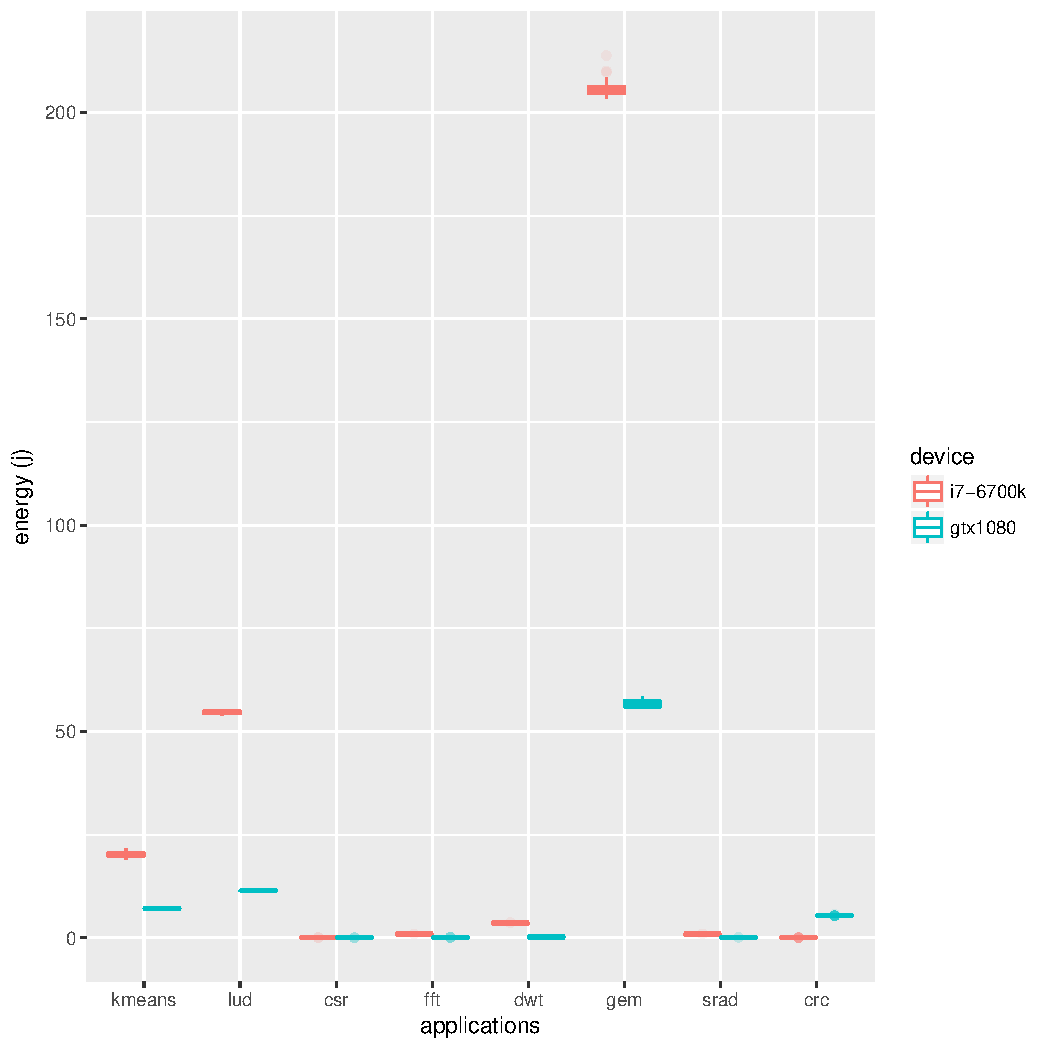
\includegraphics[width=1\textwidth]{figures/energy-results/energy_charts.pdf}
\caption{Kernel execution energy}
\label{fig:energy}
\end{subfigure}
\hfill
\begin{subfigure}{.49\textwidth}
\centering
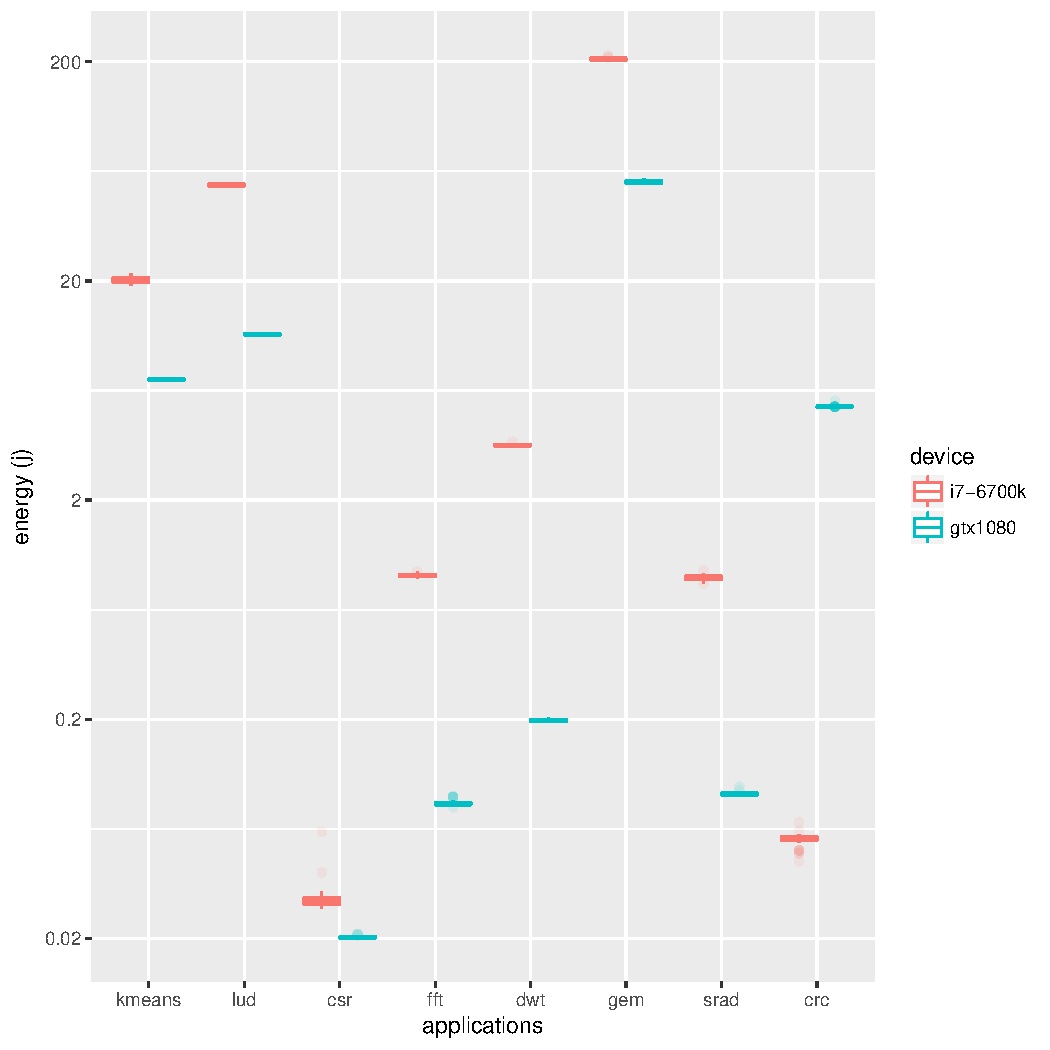
\includegraphics[width=1\textwidth]{figures/energy-results/energy_charts_log10.pdf}
\caption{Log of kernel execution energy}
\label{fig:energy-log}
\end{subfigure}
\caption{Benchmark kernel execution energy ({\bf large} problem size) on Core i7-6700K and Nvidia GTX1080}
\end{figure*}

\todo{Does energy scale with problem size for all benchmarks? Maybe not since dwarfs with large memory access cache misses could add huge overheads}

Figures~\ref{fig:energy} and~\ref{fig:energy-log} show the kernel execution energy for several benchmarks for the {\bf large} size.
All results are presented in joules.
The box plots are coloured according to device: red for the Intel Skylake i7-6700k CPU and blue for the Nvidia GTX1080 GPU.
\todo{report power as well as energy; proper analysis of the results}
The logarithmic transformation has been applied to Figure~\ref{fig:energy-log} to emphasise the variation at smaller energy scales ($<$ \SI{1}{\joule}), which was necessary due to small execution times for some benchmarks.
In future this will be addressed by balancing the amount of computation required for each benchmark, to standardize the magnitude of results.

Certain trends become apparent when directly comparing joules required over a range of problems.
All the benchmarks use more energy on the CPU, with the exception of {\tt crc} which as previously mentioned has low floating-point intensity and so is not able to make use of the GPU's greater floating-point capability. 
Variance with respect to energy usage is larger on the CPU, which is consistent with the execution time results.

\end{document}
